\begin{refsection}
	\chapter{Contexte biologique et méthodologique}

    Ce chapitre présente les notions, biologiques puis informatiques, utilisées comme fondement du travail de recherche, effectué lors de cette thèse.
    
    
    \section{Le métabolisme et sa représentation informatique}
    \subsection{Généralités sur le métabolisme}
    
    Tout organisme vivant, consomme de l'énergie afin de perpétuer son espèce. Pour cela, l'être vivant doit assimiler des composés présent dans son environnement. Ces composés chimiques permettent de produire l'énergie, nécessaire à la survie mais surtout à la transmission du patrimoine génétique. Ainsi on désigne par métabolisme, l'ensemble des processus de synthèse et dégradation de composé chimique, mis en œuvre par l'organisme. De fait, les processus comme la réplication de l'\gls{ADN}, la traduction d'un gène et autres \ldots~sont exclus.
    
    Le métabolisme est essentiel à la vie, d'une part il fournit l'énergie nécessaire. Et d'autre part, il va produire les molécules de base indispensables à l'organisme, pour sa construction, sa défense et autres \ldots 
    
    Bien qu'agissant à une échelle moléculaire, le métabolisme d'un groupe d'organisme peut impacter son environnement. Les conséquences peuvent être observées à l'échelle humaine voire dans certains cas à l'échelle de la planète (voir \ref{fig:bloom}).
    \begin{shadedfigure}
        \begin{subfigure}[b]{.5\textwidth}
            \centering
            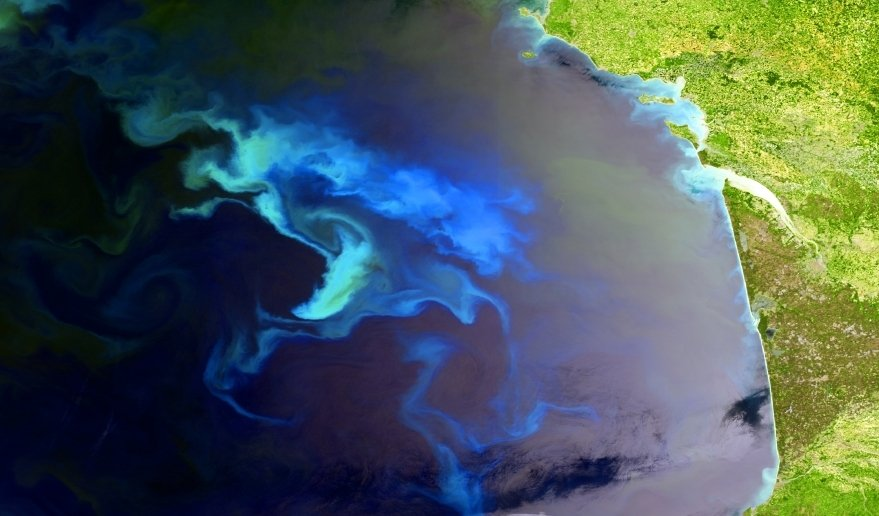
\includegraphics[width=\textwidth]{img/bloom_gascogne.jpg}
            \caption{{\tiny Source: \url{http://seos-project.eu}}}
            \label{fig:bloom_gascogne}
        \end{subfigure}
        \hfill
        \begin{subfigure}[b]{.5\textwidth}
            \centering
            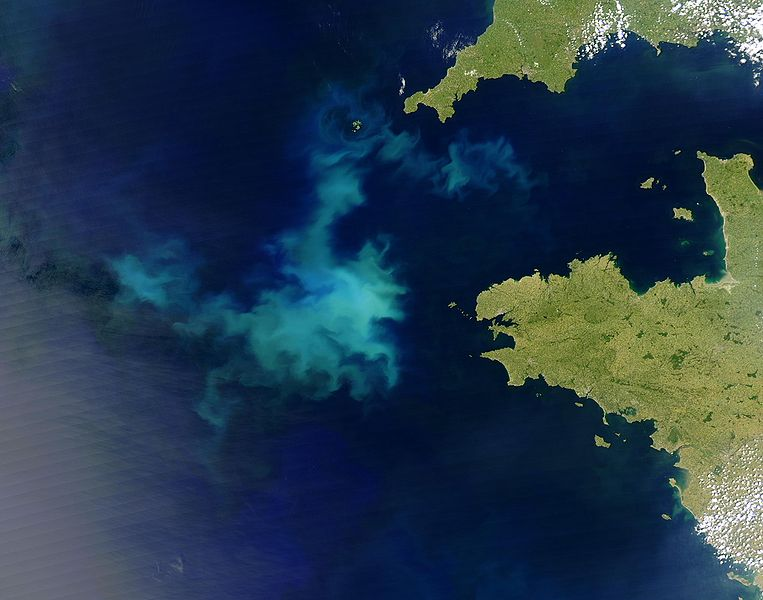
\includegraphics[width=\textwidth]{img/bloom_bretagne.jpg}
            \caption{{\tiny Source: \url{https://commons.wikimedia.org/}}}
            \label{fig:bloom_bretagne}
        \end{subfigure}
    \caption{Le métabolisme d'un groupe d'individu produit une quantité de pigment photosynthétiques suffisamment conséquente, qu'il en devient observable depuis un satellite. Deux évènements distinct sont représentés. Le premier a eu lieu au large de la Gascogne le 17 mai 2004 et le second au niveau de la Bretagne le 15 juin 2004.}
    \label{fig:bloom}
    \end{shadedfigure}

    \subsection{Les acteurs}
    
    On distingue dans le métabolisme deux catégories de processus, l'anabolisme et le catabolisme. L'anabolisme, représente l'ensemble des réactions impliqué dans la synthèse de nouvelle molécule. Au contraire, le catabolisme décrit l'ensemble des réactions de dégradation de molécule. La production de nouveaux composés nécessite de l'énergie. De tels processus sont composés de réaction endergonique. Ainsi le bilan énergétique est négatif. Par opposition, les réactions impliquées dans la dégradation d'une composé, produisent in-fine plus d'énergie qu'elles en on consommé. Les réactions produisant de l'énergie sont dites exergonique.
    
    \subsubsection{Les métabolites}
    ATP ADP energie
    
    
    \subsubsection{Les réactions}
    Ces processus s'effectuent au sein de l'organisme, dans l'infiniment petit, au niveau moléculaire. Effectivement des molécules produites par l'organisme vont avoir une affinité avec des composés chimiques. Leur rencontre provoque une transformation du composé. Puis, le ou les produits résultant de cette transformations, peuvent êtres à leur tour reconnu par des molécules produites par l'organisme. Provoquant ainsi une cascade de transformation chimique.
    
    \subsection{Représentation en graphe}
    \subsection{Ressources sur les voies métaboliques}
    \subsubsection{KEGG}
    \subsubsection{Reactome}
    \subsubsection{Unipathway}
    \subsubsection{Genome properties}
    
    \section{Des génomes aux réseaux métaboliques}
    \subsection{Annotation fonctionnelle}
    \subsection{Reconstruction des réseaux métaboliques}
    \subsection{Modèles métaboliques}
    \subsection{Les données expérimentales}
    \subsubsection{Élucidation des voies métaboliques}
    \subsubsection{Phénotypes de croissances}
    
    \section{Raisonnement logique dans le processus de curation}
    \subsection{Lacunes et incertitudes dans nos connaissances}
    \subsubsection{Les trous dans les connaissances et les enzymes orphelines}
    \subsubsection{Limites de l’annotation fonctionnelle et rôle de la curation}
    \subsection{Logique et raisonnement}
    \subsubsection{Les différentes logiques}
    \paragraph{Logique booléenne}
    \paragraph{Logique multi-valuée}
    \subsubsection{Inférence d’information}
    \paragraph{Représenation des connaissances/ontologies}
    \paragraph{Chainage avant et arrière} %backward/forward
    \paragraph{Règles et système expert}
    
    \section{Méthodes existantes}
    \subsection{HAMAP et UniRule}
    \subsection{Genome properties}
    \subsection{IMG terms}
    \subsection{HERBS}
    
    \subbibliography
\end{refsection}